\documentclass[12pt, letterpaper]{article}
\usepackage{listings}
\usepackage{graphicx}
\usepackage{color}
\usepackage{caption}
\usepackage{subcaption}
\usepackage{hyperref}
\usepackage{fancyhdr}
\usepackage{mathrsfs}
\usepackage[margin=3cm]{geometry}
\usepackage[dvips]{epsfig}
\usepackage{placeins}
\usepackage{longtable}
\usepackage{wrapfig}
\setlength{\parindent}{0.0in}
\setlength{\parskip}{0.05in}

\definecolor{dkgreen}{rgb}{0,0.6,0}
\definecolor{gray}{rgb}{0.5,0.5,0.5}
\definecolor{mauve}{rgb}{0.58,0,0.82}
\definecolor{deepblue}{rgb}{0,0,0.7}
\definecolor{deepred}{rgb}{0.6,0,0}
\definecolor{deepgreen}{rgb}{0,0.5,0}
\definecolor{red}{rgb}{0.9,0,0}

\newcommand\course{CS532}
\newcommand\semester{Spring 2017}
\newcommand\hwnum{5}
\newcommand\yourname{Justin Schaffner}
\newcommand\login{JASchaff}
\newenvironment{answer}[1]{\subsection*{Problem #1}}

\pagestyle{fancyplain}
\headheight 40pt
\lhead{\yourname\ (\login)\\\course\ --- \semester}
\chead{\textbf{\Large Assignment \hwnum}}
\rhead{\today}
\headsep 40pt
\lstnewenvironment{MyBash}{\lstset{language=bash, aboveskip=3mm, belowskip=3mm, showstringspaces=false, columns=flexible, basicstyle={\small\ttfamily}, numbers=none, numberstyle=\tiny\color{grey}, keywordstyle=\color{black}, commentstyle=\color{dkgreen}, stringstyle=\color{black}, breaklines=true, breakatwhitespace=true, tabsize=3}}{}
\lstnewenvironment{MyPython}{\lstset{language=Python, aboveskip=3mm, belowskip=3mm, basicstyle=\small, otherkeywords={self}, keywordstyle=\color{deepblue}, emph={MyClass,__init__}, emphstyle=\color{deepred}, stringstyle=\color{deepgreen}, commentstyle=\color{red}, frame=tb, showstringspaces=false, breaklines=true }}{}
\lstnewenvironment{MyR}{\lstset{language=R, aboveskip=3mm, belowskip=3mm, basicstyle=\small, breaklines=true, frame=tb}}{}

\begin{document}

\begin{answer}{1: Karate Club}
We know the result of the Karate Club (Zachary, 1977) split. Prove or disprove that the result of split could have been predicted by the weighted graph of social interactions.\\
One of the links from the assignment, \url{https://networkx.readthedocs.io/en/stable/examples/graph/karate_club.html} , gives a quick way to get the data from the Karate Club study found here: \url{http://aris.ss.uci.edu/~lin/76.pdf}. Adjustments to the short python script allow the data to be easily worked in R.\\
\begin{MyPython}
import networkx as nx
G=nx.karate_club_graph()
nx.write_graphml(G, 'karate_club.graphml')
\end{MyPython}
This creates a graphml file in the working folder containing the network graph of the Karate Club study.\\
According to the original study, Zachary used a program called NETFLOW which implements the network flow algorithm developed by Ford and Fulkerson in 1962. Network flow along edges is based on the number of shortest paths that utilize each edge. Edges with the highest flow represent bridges between possible communities within the larger community. In the Karate Club study, the predicted split between the officers and Mr. Hi was accurate for all members except one whose choice was based on factors other than social connnections.\\
In R, the igraph libary contains the cluster\textunderscore edge\textunderscore betweeness() function which operates on a similar principle to NETFLOW. Using cluster\textunderscore edge\textunderscore betweeness() I was able to generate the community graph in Figure 1.
\FloatBarrier
\begin{wrapfigure}{l}{0.53\linewidth}
\caption{}
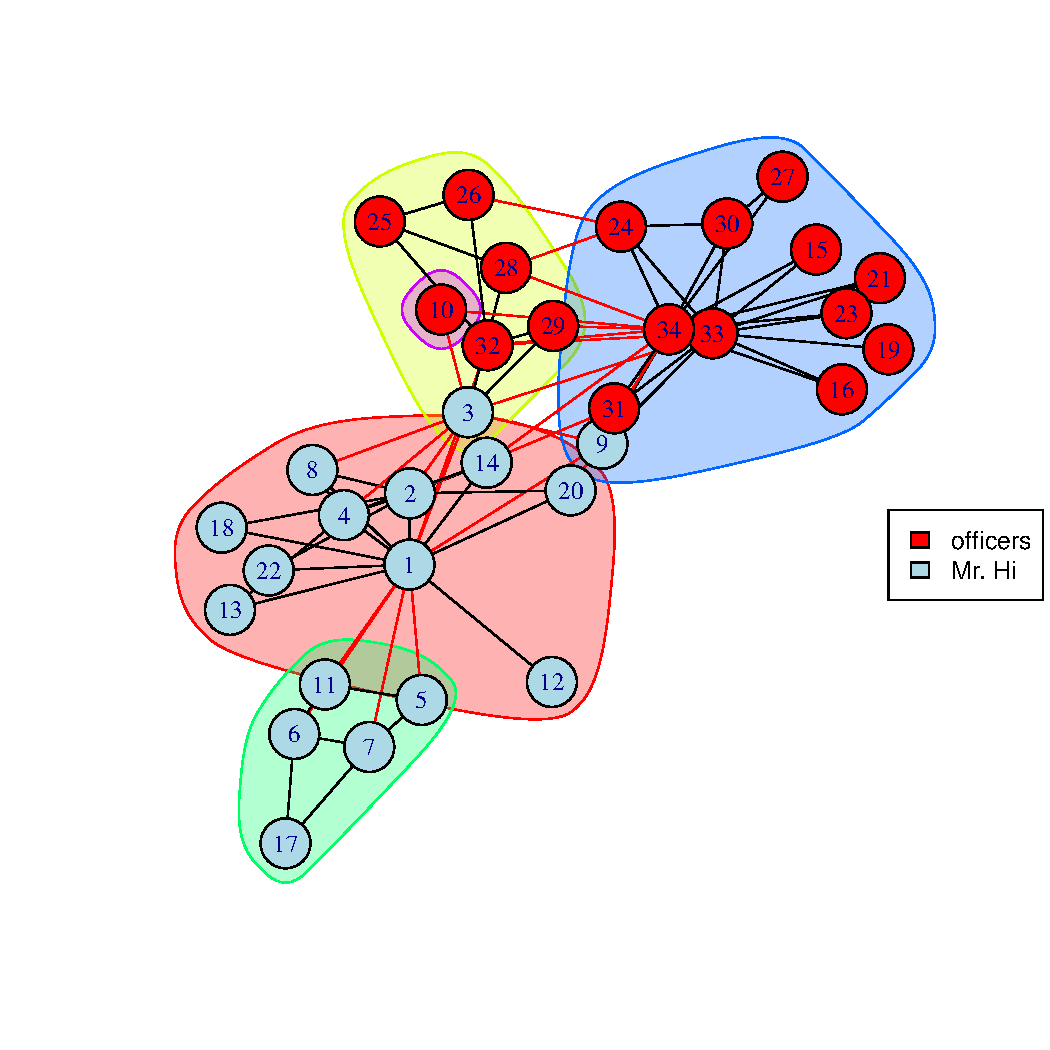
\includegraphics[trim=0 50 0 50, clip, width=\linewidth]{karate_club_cluster_edge_2}
\end{wrapfigure}

The vertices are colored based on their final membership decision when the club split. The R function divided the group into 4 smaller communities, with one loner, number ten. Two core communities can be identified, with strong central characters, one based around number 1 vertice, and the second around vertices 33 and 34. As in the original study, number 9 seems to be in the officers camp, but with some overlap with Mr. Hi's. In the data from Zachary, number 9 professed weak ties with the officers, and ultimately chose Hi . Number 20 seems to be in a similar but reversed position, with weak ties to Mr. Hi. In the original study, the data collected showed that number 20 did have weak ties to Mr. Hi, which is reflected in its weak association with that community. The two sub communities apart form the core communities for the most part show strong ties with one faction or the other. In each sub group there is one individual, 17 or 25,  who appears to have none or weak ties to either of the factions, but is attached to people who do have strong factional alliances. The data from the study shows that Number 3 has strong ties to Mr. Hi, but due to some of their extra-club associations, the algorithm placed 3 in a subgroup which has strong Officer ties, but it also placed 3 in the core group belonging to Mr. Hi. The loner, number 10, showed no factional alighnment prior to the split, and does not seem to have many strong associations with club members outside of club activities. Since one of its two connections is with one of the officers, the algorithm placed 10 in its own community within the sub Officer community. For each case, the algorithm placed the individuals either with the core group they eventually chose or within a subgroup closely associated with that core group, the only exception being number 9, which the algorithm placed slightly on the Officer side of the fence, but proved to make the choice to go with Mr. Hi. If you count 9 as a total miss, then the miss rate for the algorithm for this study would be 2.9\% .
\FloatBarrier
\begin{longtable}{lll}
\small
\caption{Original Data from Karate Club Study}\\
Individual  & Faction  & Club\\ \hline
1  & Hi-Strong  & Hi\\
2  & Hi-Strong  & Hi\\ 
3  & Hi-Strong  & Hi\\
4  & Hi-Strong  & Hi\\
5  & Hi-Strong  & Hi\\
6  & Hi-Strong  & Hi\\
7  & Hi-Strong  & Hi\\
8  & Hi-Strong  & Hi\\
9  & Officer-Weak  & Hi\\
10  & None  & Officer\\
11  & Hi-Strong  & Hi\\
12  & Hi-Strong  & Hi\\
13  & Hi-Weak  & Hi\\
14  & Hi-Weak  & Hi\\
15  & Officer-Stron  & Officer\\
16  & Officer-Weak  & Officer\\
17  & None  & Hi\\
18  & Hi-Weak  & Hi\\
19  & None  & Officer\\
20  & Hi-Weak  & Hi\\
21  & Officer-Strong  & Officer\\
22  & Hi-Weak  & Hi\\
23  & Officer-Strong  & Officer\\
24  & Officer-Weak  & Officer\\
25  & Officer-Weak  & Officer\\
26  & Officer-Strong  & Officer\\
27  & Officer-Strong  & Officer\\
28  & Officer-Strong  & Officer\\
29  & Officer-Strong  & Officer\\
30  & Officer-Strong  & Officer\\
31  & Officer-Strong  & Officer\\
32  & Officer-Strong  & Officer\\
33  & Officer-Strong  & Officer\\
34  & Officer-Strong  & Officer

\end{longtable}
\FloatBarrier
I also tested the data with the cluster\textunderscore leading\textunderscore eigen() function in the igraph library with the results shown in Figure 2.
\FloatBarrier
\begin{wrapfigure}{l}{0.53\linewidth}
\caption{}
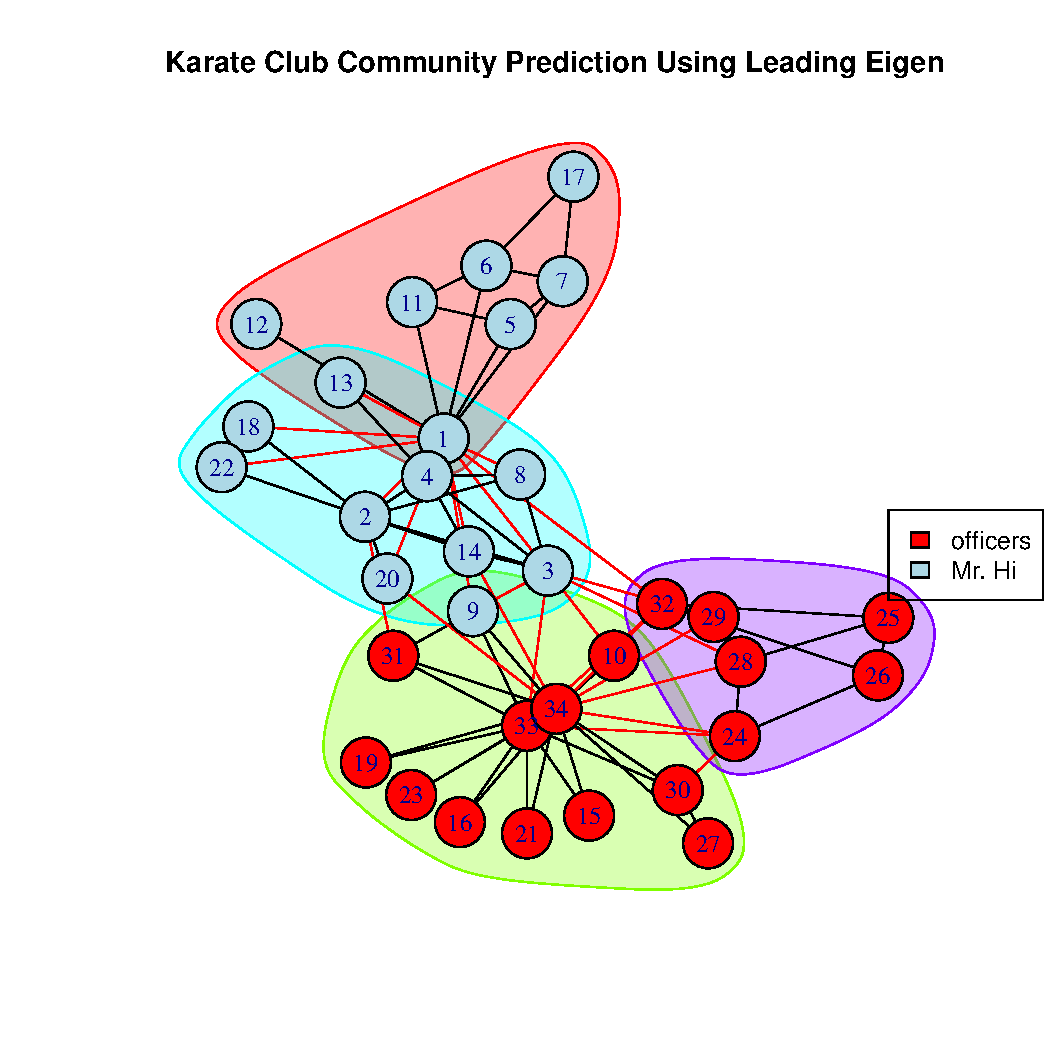
\includegraphics[trim=0 50 0 50, clip, width=\linewidth]{karate_club_cluster_eigen_2}
\end{wrapfigure}

The difference between the results of the two methods appear minimal, but there is less ambiguity in the eigen predictions for some of those who were borderline for the betweenness function. 9 is caste as a member of both core communities, while the other numbers seem to be more firmly associated with the core group they eventually chose. Most of the differences occur in how the algorithm split the subgroups from the core groups. 24 is now a part of the Officers sub group, while 3 is excluded and is more firmly associated with Mr. Hi. 12 has been placed in Mr. Hi's subgroup despite the fact that 12 has no relationships with anyone within the sub group and has strong ties to Mr. Hi. 12 was placed in this group based on eigen vector values compared to that of the other members by their signs. In this case, that doesn't necessarily imply social interaction between community members. 10 has also not been marked out as a loner. While being less ambiguous in its results, the eigen function may be missleading in how it selects its communities, if 12 is an indicator. Despite the differences, if used to predict the factional split, with 9 counted as a miss since its decision seems to be 50/50 either way, the miss rate would still be 2.9\% . For this study, the final split could have been predicted with a 97\% accuracy with either of these methods.
\newpage
The R code for Figure 1:
\begin{MyR}
require(graphics)
library(igraph)

pdf('Desktop/karate_club_cluster_edge_2.pdf')
karate_graph<-read.graph('Desktop/karate_club.graphml', format='graphml')
karate_eb<-cluster_edge_betweenness(karate_graph)
colors<-c('light blue', 'light blue', 'light blue', 'light blue', 'light blue', 'light blue', 'light blue', 'light blue', 'light blue', 'red', 'light blue', 'light blue', 'light blue', 'light blue', 'red', 'red', 'light blue', 'light blue', 'red', 'light blue', 'red', 'light blue', 'red', 'red', 'red', 'red', 'red', 'red', 'red', 'red', 'red', 'red', 'red','red')
plot(karate_eb, karate_graph, col=colors)
legend(x=0, legend=c("officers", "Mr. Hi"), fill=c('red', 'light blue'))
dev.off()
\end{MyR}
The R code for Figure 2:
\begin{MyR}
require(graphics)
library(igraph)

pdf('Desktop/karate_club_cluster_eigen_2.pdf')
karate_graph<-read.graph('Desktop/karate_club.graphml', format='graphml')
karate_eb<-cluster_leading_eigen(karate_graph)
colors<-c('light blue', 'light blue', 'light blue', 'light blue', 'light blue', 'light blue', 'light blue', 'light blue', 'light blue', 'red', 'light blue', 'light blue', 'light blue', 'light blue', 'red', 'red', 'light blue', 'light blue', 'red', 'light blue', 'red', 'light blue', 'red', 'red', 'red', 'red', 'red', 'red', 'red', 'red', 'red', 'red', 'red','red')
plot(karate_eb, karate_graph, col=colors, main="Karate Club Community Prediction Using Leading Eigen")
legend(x=0, legend=c("officers", "Mr. Hi"), fill=c('red', 'light blue'))
dev.off()
\end{MyR}
\end{answer}
\end{document}
